\section{Design of the Delay and \gls{reverb} Effect}
In this section, the delay and the \gls{reverb} will be designed to fit into a \gls{dsp}, which means that a discreet block diagram is obtained and afterwards the differential equations to implement in the \gls{dsp} will be made. The effects will be simulated in MATLAB and then the assembly code will be developed and implemented. 


\subsection{Obtaining the Differential Equation}\label{sec:reverb_develop}
The Delay effect is a simpler version of the \gls{reverb} effect and therefore they will be presented and designed in the same section. The block diagram presented in \autoref{sec:reverberation} \autoref{fig:reverb_block} is changed so it fits into a direct form 1 and 2 construction.
A way to design a \gls{reverb}, which imitates the natural reverberation of a room, is with a serial connection of two blocks. The first block is a parallel connection of \gls{lpcf}, and the second block is a serial connection of allpass filters \citep{natural_sounding_revorb}. 
The \gls{lpcf} is used because the room acoustic characteristics is acting as a low pass filter. All low frequency signals will stay longer in the room than the high frequency \citep{rfi}. The \gls{reverb} needs to have at least 1000 echo per second, and this can be obtained with six \gls{lpcf} filters in parallel, and two all pass filter afterwords in serial \citep{DAFX}. Otherwise if there was not two all pass filters afterwords, it would require 40 \gls{lpcf} to make 1000 echo per second \citep{natural_sounding_revorb}. The all pass filter in \autoref{fig:reverb_block_des} is in direct form 2 because of the delay length. The delay effect and some of the \gls{reverb} effect is shown in \autoref{fig:reverb_block_des}. The \gls{reverb} effect is both the one in red and black while the delay is only the red block. 

\newpage

\begin{figure} [htbp]
 \centering
\begin{picture}(0,0)%
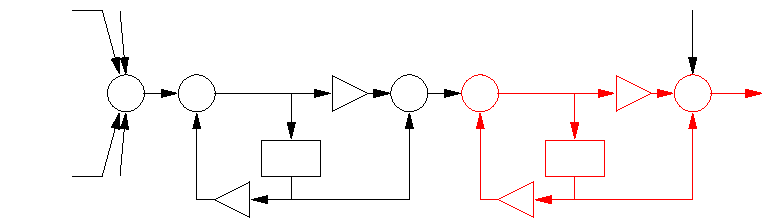
\includegraphics{reverb_diag_des.pdf}%
\end{picture}%
\setlength{\unitlength}{4144sp}%
%
\begingroup\makeatletter\ifx\SetFigFont\undefined%
\gdef\SetFigFont#1#2#3#4#5{%
  \reset@font\fontsize{#1}{#2pt}%
  \fontfamily{#3}\fontseries{#4}\fontshape{#5}%
  \selectfont}%
\fi\endgroup%
\begin{picture}(5832,1599)(-1319,-1288)
\put(3601,209){$x[n]$}%
\put(2656,-106){\color[rgb]{1,0,0}$w_8[n]$}%
\put(1711,-421){$\Sigma$}%
\put(721,-916){$z^{-d_7}$}%
\put( 91,-421){$\Sigma$}%
\put(1261,-196){$-\alpha$}%
\put(2251,-421){\color[rgb]{1,0,0}$\Sigma$}%
\put(2881,-916){\color[rgb]{1,0,0}$z^{-d_8}$}%
\put(271,-1006){$\alpha$}%
\put(2431,-1006){\color[rgb]{1,0,0}$\alpha$}%
\put(3871,-421){\color[rgb]{1,0,0}$\Sigma$}%
\put(3421,-196){\color[rgb]{1,0,0}$-\alpha$}%
\put(-449,-421){$\Sigma$}%
\put(-224,-106){$x_7[n]$}%
\put(1936,-106){\color[rgb]{1,0,0}$x_8[n]$}%
\put(4276,-106){\color[rgb]{1,0,0}$y[n]$}%
\put(-1304,-151){LPCF}%
\put(-1304,-421){filter in}%
\put(-1304,-646){Parallel}%
\end{picture}%

  \caption{The figure shows some of a block diagram of a \gls{reverb} (black and red) and the delay unit (red).}
  \label{fig:reverb_block_des}
\end{figure}

From \autoref{fig:reverb_block_des}, the following differential equations \autoref{eq:delay_eq_sub} can be derived for the delay effect, where the index 8 is omitted since the delay effect only is the red all pass filter, $x[n] = x_8[n]$ and $w[n] = w_8[n]$.

\begin{subequations}\label{eq:delay_eq_sub}
\begin{equation}\label{eq:delay_eq}
       y[n] = - \alpha \cdot w[n] + w[n-d]
    \end{equation}
\begin{equation}\label{eq:delay_eq_in}
       w[n] = \alpha \cdot w[n-d] + x[n] 
    \end{equation}
 \end{subequations}
		
		

The \gls{reverb} unit is more advanced than the delay unit and before the differential equations can be derived, some calculations are needed. The \gls{reverb} unit calculations are based on an article \citep{natural_sounding_revorb} which explain the design parametric for a Schroeder \gls{reverb} processor unit. From \citep{natural_sounding_revorb} the \gls{reverb} time is defined by \autoref{eq:reverb_defined}.



\begin{equation}
\label{eq:reverb_defined}
		T = \frac{60}{-20 \cdot log(\alpha)} \cdot \tau
\end{equation}

    \startexplain
\explain{$60$ is the \gls{reverb} attenuation in \si{\decibel}}{\si{\decibel}}
\explain{$\tau$ is the delay time}{\si{\second}}
\explain{$T$ is \gls{reverb} time, which is the time it takes for a signal to be attenuated \SI{60}{\decibel}}{\si{\second}}
\explain{$-20 \cdot log10(\alpha)$ is the attenuation in the feedback loop for each round}{\si{\decibel}}
    \stopexplain

Both the positive and negative gain $\alpha$ is defined to be 0.708  \citep{natural_sounding_revorb} and the total \gls{reverb} echo density shall at lest be 1000 echo per second. In \autoref{eq:reverb_defined_tal_res} it can be obtained that $\tau$ shall be $\frac{1}{20}$ of $T$, with $T$= \SI{1}{\second}.


\begin{subequations}
\begin{equation}\label{eq:reverb_defined_tal}
       T = \frac{60}{-20 \cdot log10(0.708)} \cdot \tau
       \addunit{\si{\second}}
    \end{equation}
\centering
$\Updownarrow$
\begin{equation}\label{eq:reverb_defined_tal_res}
        \tau = \frac{1}{20} T
        \addunit{\si{\second}}
    \end{equation}
 \end{subequations}

\autoref{eq:reverb_defined_tal_res} then shows that $\tau$ is \SI{50}{\milli\second} with a total \gls{reverb} time $T$ of \SI{1}{second}. This gives an echo density of 20 echoes per second for each of the \gls{lpcf}, but if all the filters have the same delay time, some echoes will interfere. To avoid interference each filter delay time is chosen to its own prime number, which is shorter than \SI{50}{\milli\second}. The chosen delay prime numbers are as in \autoref{tab:reverb_delay}, six for the \gls{lpcf}s and two for the the allpass filter, so it is possible to design a Moorer \gls{reverb} unit \citep{DAFX}. 

\begin{table}[htbp]
\centering
\caption{The chosen delay prime numbers}
\label{tab:reverb_delay}
\begin{tabular}{llllll}
$d_1$ & = & 19 & $d_5$ & = & 37 \\ 
$d_2$ & = & 23 & $d_6$ & = & 41 \\
$d_3$ & = & 29 & $d_7$ & = & 17 \\
$d_4$ & = & 31 & $d_8$ & = & 13
\end{tabular}
\end{table}

%The same applies in the chose of \autoref{tab:reverb_bgain}.
%Each \gls{lpcf} filter is also attenuated by a defined gain which is shown in \autoref{tab:reverb_bgain}
%
%\begin{table}[htbp]
%\centering
%\caption{The chosen gain in \gls{lpcf}}
%\label{tab:reverb_bgain}
%\begin{tabular}{lll}
%$b_1$ & = & 1 \\
%$b_2$ & = & 0.9 \\
%$b_3$ & = & 0.8 \\
%$b_4$ & = & 0.7 \\
%$b_5$ & = & 0.6 \\
%$b_6$ & = & 0.5 
%\end{tabular}
%\end{table}


The \gls{reverb} unit requires 1000 echoes per second \citep{natural_sounding_revorb}. To achieve a natural \gls{reverb} sound, multiple all pass filter delay units have to be connected in serial after the six \gls{lpcf} in parallel. It is defined by \citep{natural_sounding_revorb} that two all pass filter is required to make a natural \gls{reverb} sound.
To calculate the approximated number of echoes in one second from six \gls{lpcf}, the following calculations are made. The total numbers of echoes over \SI{-60}{\decibel} is added together from each \gls{lpcf} filter because each \gls{lpcf} has its own prime number. The result is maximum $6 \cdot 20 = 260$ echoes per second. The reason of this is that each \gls{lpcf} makes 20 echoes that is above \SI{-60}{\decibel}. The number of echoes from the six \gls{lpcf}'s is different from the number of outputs from the six \gls{lpcf}'s, because a direct input is sent through each \gls{lpcf}, which is not counted as an echo. These six direct inputs arrives at the same time, so they are counted as one output. The number of outputs from each \gls{lpcf} is therefore 21, and the maximum number of outputs from the six parallel \gls{lpcf}'s is $6 \cdot 20 + 1 = 261$.  In \autoref{fig:reverb_block_design} it is seen that each \gls{lpcf} is followed by an individual gain called $b_1$ to $b_6$. These gain values are chosen as in \autoref{tab:reverb_bgain}

\begin{table}[htbp]
\centering
\caption{The chosen gain in \gls{lpcf}}
\label{tab:reverb_bgain}
\begin{tabular}{lll}
$b_1$ & = & 1 \\
$b_2$ & = & 0.9 \\
$b_3$ & = & 0.8 \\
$b_4$ & = & 0.7 \\
$b_5$ & = & 0.6 \\
$b_6$ & = & 0.5 
\end{tabular}
\end{table}

This means that only the \gls{lpcf} with $b = 1$ will produce 20 echoes above \SI{-60}{\decibel}. The \gls{lpcf}s where $b$ is less than one will therefore reach the \SI{-60}{\decibel} limit faster, and will therefore produce less echoes above \SI{-60}{\decibel}.
As seen in \autoref{fig:reverb_block_design} the output of the six \gls{lpcf} is then sent through two allpass filters. The number of echoes after the first allpass filter can be found from a simulation in MATLAB. The simulation is done with a serial connection of only one \gls{lpcf} and one allpass filter. It is then checked how many outputs of the allpass filter above \SI{-60}{\decibel} the circuit will produce.  
This simulation is done six times, where the gain of the \gls{lpcf} is changed each time. The first simulation e.g. is when $b = b_1$. Here it is seen that 210 outputs will be produced, before the \SI{-60}{\decibel} limit is reached. The number 210 is found from that when an input is sent to the \gls{lpcf}, the \gls{lpcf} will produce 21 outputs above \SI{-60}{\decibel}. Then when the first output of the \gls{lpcf} is made as the input to the allpass filter, the allpass filter will produce 20 outputs. The second output from the \gls{lpcf} will produce 19 outputs from the allpass filter. It appears that the number of outputs from a single \gls{lpcf} and a single allpass filter can be expressed as in \autoref{eq:rev_out_gen}.

\begin{equation}\label{eq:rev_out_gen}
        y = \sum_{x=1}^{m} x
        \addunit{\si{1}}
    \end{equation} 
    
    \startexplain
\explain{$y$ is the total number of outputs from a single \gls{lpcf} and a single allpass filter}{\si{1}}
\explain{$m$ is the maximum number of outputs from the allpass filter, with a single output from the \gls{lpcf}, as the input}{\si{1}}
    \stopexplain

$m$ in \autoref{eq:rev_out_gen} changes as the \gls{lpcf} gain, $b$, changes. For $m = 20 \big|_{b=b_1}$, $m = 19 \big|_{b=b_2 \ and \ b=b_3}$, $m = 18 \big|_{b=b_4 \ and \ b=b_5}$, and $m = 17 \big|_{b=b_6}$.  
The total number of outputs from the six \gls{lpcf} in parallel, followed by an allpass filter i serial, can then be found as in \autoref{}.

\begin{subequations}
\begin{equation}\label{eq:reverb_ser}
      \text{Echo} + \text{direct sound} = \sum_{x=1}^{20} x + \sum_{x=1}^{19} x + \sum_{x=1}^{19} x + \sum_{x=1}^{18} x+ \sum_{x=1}^{18} x+ \sum_{x=1}^{17} x -5
    \end{equation}
\centering
$\Updownarrow$
\begin{equation}\label{eq:reverb_seriel}
        \text{Echo} + \text{direct sound}= 1080
        \addunit{\si{1}}
    \end{equation}
 \end{subequations}

The subtraction of five in \autoref{eq:reverb_ser} is, as mentioned earlier, because each \gls{lpcf} sends through a direct input, which arrives at the same time, and is therefore counted as one output.
The second allpass filter in \autoref{fig:reverb_block_design} is set to have the same parameters as the first allpass filter. There only a few requirements for the second allpass filter, because the number of echoes is already higher than 1000. Therefore the only requirements for the second allpass filter is that it has to be an allpass filter and it must not decrease the number of echoes. This is fulfilled by copying the first allpass filter. 
    
%
%\includeCode{echo_1_all_pass.m}{matlab}{6}{23}{The reverb echo calcul6ation matlab code}{code:reverb_cal}{code/design/}

%The output plot from the \gls{reverb} code where the input is guided through the upper \gls{lpcf} and afterwards through the first all pass filter is as following \autoref{fig:reverbcal_plot}. This plot shows only one echo from the all pass filter the blue line and the output of this pulse from the first all pass filter, the red line.
%
%\begin{figure}[htbp]
%	\centering
%	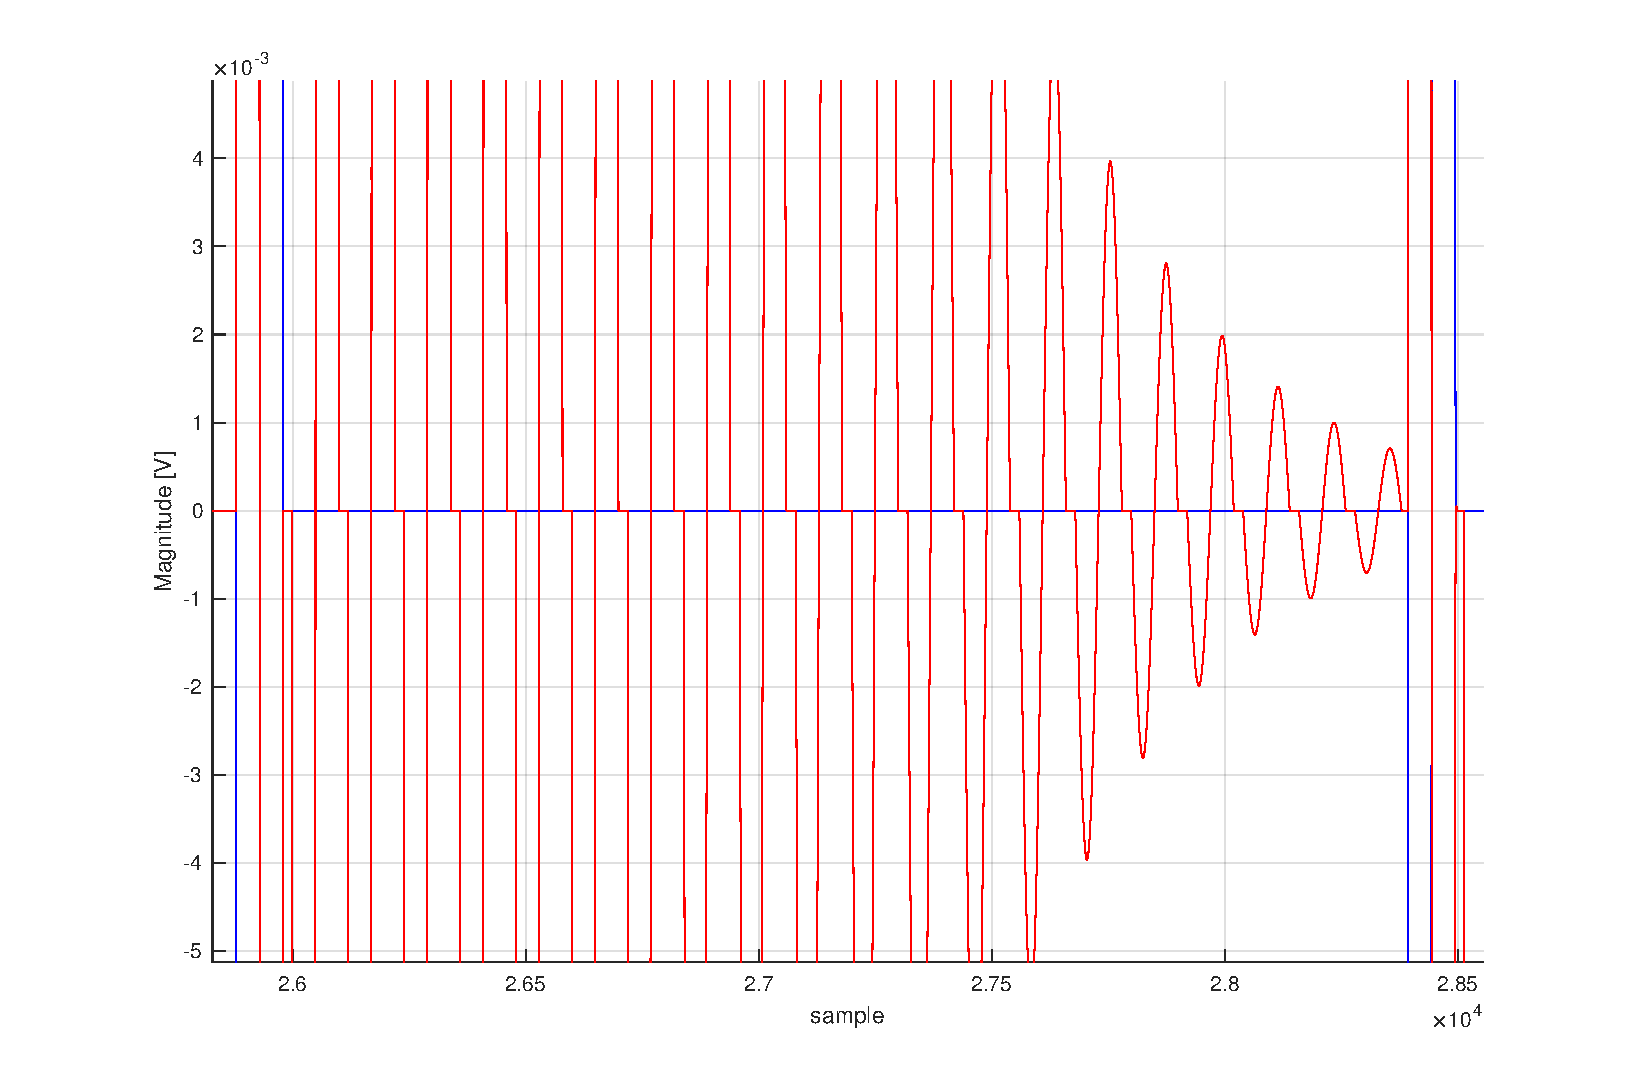
\includegraphics[width=0.9\textwidth]{reverbcal}
%	\caption{The plot shows the direct sound plus 19 echo }
%	\label{fig:reverbcal_plot}
%\end{figure}

%Form the MATLAB script \autoref{code:reverb_cal} the formula of calculation echo after the first all pass filter is as following \autoref{eq:reverb_ser}. The $-5$ is included because only one of the direct sound is taken to acound in the formula.

In \citep{DAFX} Moorer suggests adding an early reflection network before the six \gls{lpcf}s. The early reflection network is a simple multi tap \gls{fir} filter constellation. Moorer also suggests making the \gls{lpcf} feedback gain as a variable, so the user can change the room size and damping. To design the \gls{lpcf} filter the standard comp filter needs to be changed  \citep{LPCFfd}. The standard comb filter have the following transfer function \autoref{eq:comb_filter}

\begin{equation}\label{eq:comb_filter}
H(z)=\frac{1}{1-c \cdot z^{-d}}
\end{equation}

    \startexplain
\explain{$a$ is the amplification of the combs }{\si{1}}
    \stopexplain

To change the comb filter caracteristics, so the magnitude in the high frequency is lower than the magnitude in the low frequency, $a$ needs to be changed to a low pass filter. \\

In the frequency domain, the low pass filter have the following transfer function \autoref{eq:comb_filter_freq} 


\begin{equation}\label{eq:comb_filter_freq}
	G(s) = f \cdot \frac{\omega_{0}}{s+w_{0}}
\end{equation}

\autoref{eq:s2z} will be used in order to pass from the $frequency$ to the $z-domain$:

\begin{equation}\label{eq:s2z}
	s = \frac{1-z^{-1}}{T}
\end{equation}

Where:

$T$ is the sampling time, the inverse of the sampling frequency $f_{s}$. \\

By inserting \autoref{eq:s2z} into \autoref{eq:comb_filter_freq}, \autoref{eq:s2z2} is obtained:

\begin{equation}\label{eq:s2z2}
	G(z) = f \cdot \frac{\omega_{0}}{\frac{1 - z^{-1}}{T} + \omega_{0}}
\end{equation}

Which also gives:

\begin{equation}
	G(z) = f \cdot \frac{\frac{\omega_{0} \cdot T}{1 + \omega_{0} \cdot T}}{1 - \frac{1}{1+ \omega_{0} \cdot T} \cdot z^{-1}}
\end{equation}

The numerator is an expression containing only constants which will be represented by $b$. The same goes for the coefficient of $z^{-1}$ in the denominator which will be represented by $a$. \autoref{eq:before_final} is then obtained:

\begin{equation}\label{eq:before_final}
	G(z) = f \cdot \frac{b}{1 - a \cdot z^{-1}}
\end{equation}

Adding $a$ and $b$ gives 1, the following relation between $a$ and $b$ can be inferred:

\begin{equation}
	b = 1 - a
\end{equation} 

\autoref{eq:before_final} can be re-written as:

\begin{equation}\label{eq:comb_filter_lp}
G(z)=f \frac{1-a}{1-a \cdot z^{-1}}
\end{equation}
  
Recalling \autoref{eq:comb_filter} and replacing $c$ by $G(z)$ from \autoref{eq:comb_filter_lp}, the final transfer function of the \gls{lpcf} is in \autoref{eq:comb_filter_lp_final}

 \begin{equation}\label{eq:comb_filter_lp_final}
H(z)=\frac{1}{1-f \frac{1-a}{1-a \cdot z^{-1}} \cdot z^{-d}}
\end{equation}

 The following \autoref{eq:reverb_eq_eks} shows the differential equation for the \gls{lpcf}'s. 

    \begin{equation}\label{eq:reverb_eq_eks}
        x_2[n] = x_1[n] - L_D \cdot x_1[n-1] + L_D \cdot x_2[n-1] + f \cdot (1-L_D) \cdot x_2[n-d_1]
    \end{equation}
    
    \startexplain
\explain{$f$ is defining the room size}{\si{1}}
    \stopexplain

$f$ is found as described in \autoref{eq:reverb_eq_f}, where scaleroom is used to scale the room size by the user \citep{LPCFfd}.

\begin{subequations}\label{eq:reverb_eq_f}
\begin{equation}\label{eq:reverb_eq_f1}
    f = \text{roomsize} = \text{initialroom} \cdot \text{scaleroom} + \text{offsetroom}
    \end{equation}
\centering
%$\Updownarrow$
\begin{equation}\label{eq:reverb_eq_f2}
    f = 0.5 \cdot \text{scaleoom} + 0.7
    \end{equation}
 \end{subequations}   
   
The $L_D$ is defining the room damping, and the equation for $L_D$ is as in \autoref{eq:reverb_eq_L_D}, where scaledamp is used to scale the room damping by the user \citep{LPCFfd}.    

\begin{subequations}\label{eq:reverb_eq_L_D}
\begin{equation}\label{eq:reverb_eq_L_D1}
    L_D = \text{damp} = \text{initialdamp} \cdot \text{scaledamp}
    \end{equation}
\centering
%$\Updownarrow$
\begin{equation}\label{eq:reverb_eq_L_D2}
    L_D = 0.5 \cdot \text{scaledamp}
    \end{equation}
 \end{subequations}   

This transfer function is plotted in MATLAB with a sweep from \SI{16}{\hertz} to \SI{20}{\kilo\hertz} and gives the following result \autoref{fig:lpcf_sweep}, where the red sine wave is the input and the blue sine wave is the output.

\begin{figure}[htbp]
	\centering
	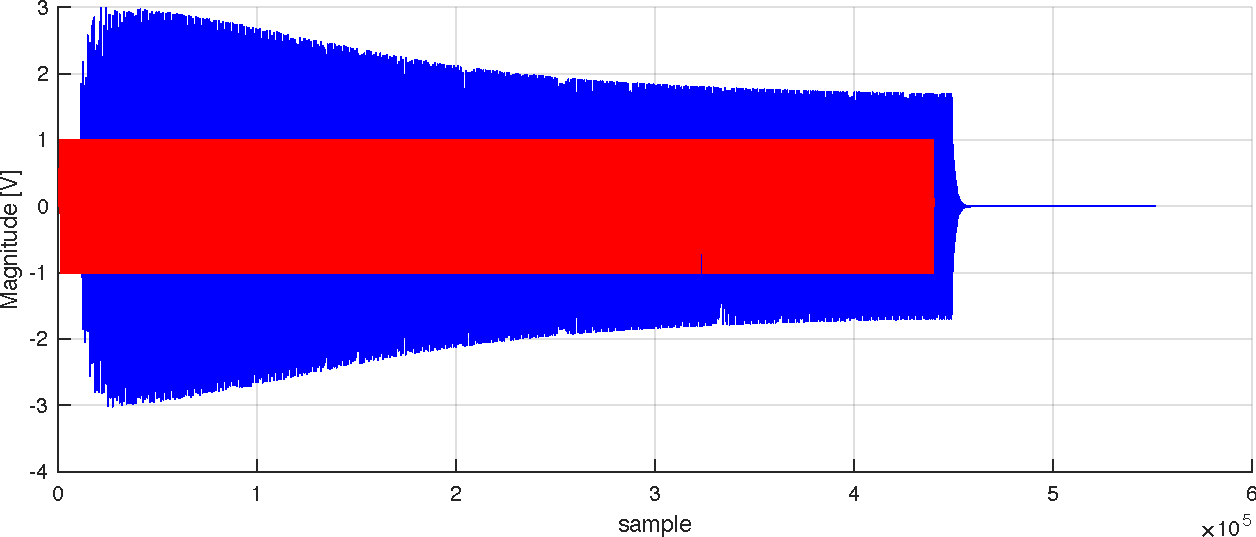
\includegraphics[width=0.6\textwidth]{lpcf_sweep}
	\caption{The plot shows the result for a sweep from \SI{16}{\hertz} to \SI{20}{\kilo\hertz} of the \gls{lpcf}}
	\label{fig:lpcf_sweep}
\end{figure}

   The following \autoref{fig:reverb_block_design} shows the block diagram over the \gls{reverb} unit, where $g = f \cdot (1-L_D)$.

\begin{figure} [htbp]
 \centering
\begin{picture}(0,0)%
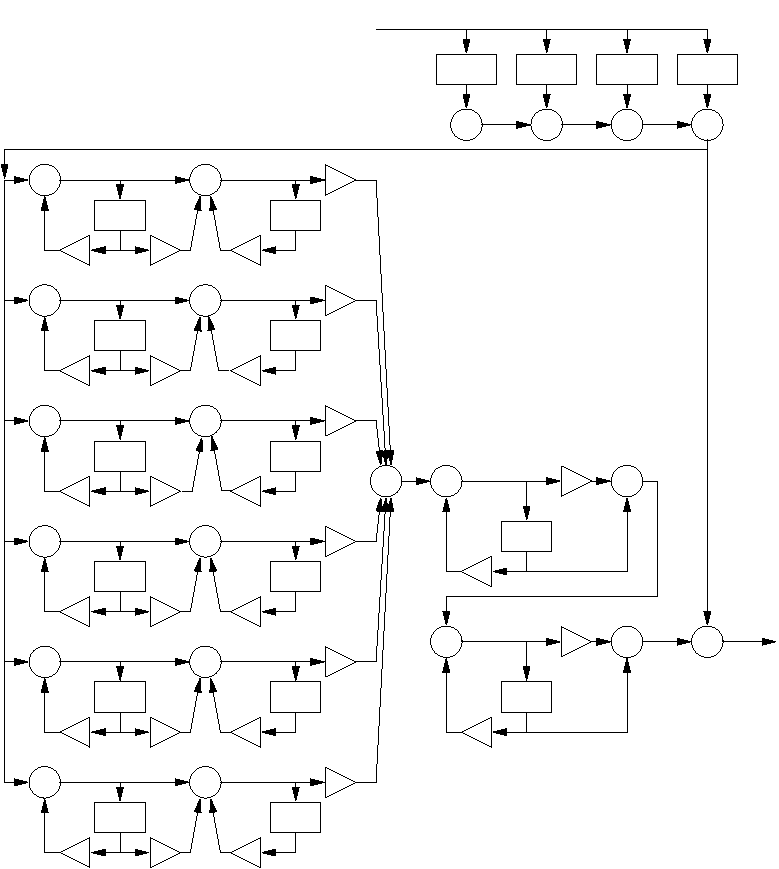
\includegraphics{reverb_serial_des.pdf}%
\end{picture}%
\setlength{\unitlength}{3646sp}%
%
\begingroup\makeatletter\ifx\SetFigFont\undefined%
\gdef\SetFigFont#1#2#3#4#5{%
  \reset@font\fontsize{#1}{#2pt}%
  \fontfamily{#3}\fontseries{#4}\fontshape{#5}%
  \selectfont}%
\fi\endgroup%
\begin{picture}(6819,10935)(-3656,-5764)
\put(541,-1681){$w_9[n]$}%
\put(1711,-421){$\Sigma$}%
\put(721,-916){$z^{-d_7}$}%
\put( 91,-421){$\Sigma$}%
\put(1261,-196){$-\alpha$}%
\put(271,-1006){$\alpha$}%
\put(-449,-421){$\Sigma$}%
\put(-224,-106){$x_8[n]$}%
\put( 91,-1861){$\Sigma$}%
\put(1711,-1861){$\Sigma$}%
\put(271,-2446){$\alpha$}%
\put(721,-2356){$z^{-d_8}$}%
\put(1261,-1636){$-\alpha$}%
\put(2701,-1636){$y[n]$}%
\put(2431,-1861){$\Sigma$}%
\put(-764,-2941){$b_5$}%
\put(-764,-4741){$b_6$}%
\put(-764,-1141){$b_4$}%
\put(-764,659){$b_3$}%
\put(-764,2459){$b_2$}%
\put(-764,4259){$b_1$}%
\put(-2519,4079){$\Sigma$}%
\put(-1844,4394){$z^{-d_1}$}%
\put(-1394,4259){$x_2[n]$}%
\put(-3374,3764){$z^{-1}$}%
\put(-1844,3764){$z^{-1}$}%
\put(-2204,4889){$g$}%
\put(-2519,2279){$\Sigma$}%
\put(-1394,2459){$x_3[n]$}%
\put(-1844,2594){$z^{-d_2}$}%
\put(-1844,1964){$z^{-1}$}%
\put(-3374,1964){$z^{-1}$}%
\put(-2204,3089){$g$}%
\put(-1844,794){$z^{-d_3}$}%
\put(-1394,659){$x_4[n]$}%
\put(-1844,164){$z^{-1}$}%
\put(-2519,479){$\Sigma$}%
\put(-3374,164){$z^{-1}$}%
\put(-2204,1289){$g$}%
\put(-2519,-1321){$\Sigma$}%
\put(-1844,-1006){$z^{-d_4}$}%
\put(-1394,-1141){$x_5[n]$}%
\put(-1844,-1636){$z^{-1}$}%
\put(-3374,-1636){$z^{-1}$}%
\put(-2204,-511){$g$}%
\put(-2519,-3121){$\Sigma$}%
\put(-1844,-3436){$z^{-1}$}%
\put(-1844,-2806){$z^{-d_5}$}%
\put(-3374,-3436){$z^{-1}$}%
\put(-2204,-2311){$g$}%
\put(-1394,-2941){$x_6[n]$}%
\put(-2519,-4921){$\Sigma$}%
\put(-1844,-5236){$z^{-1}$}%
\put(-1844,-4606){$z^{-d_6}$}%
\put(-1394,-4741){$x_7[n]$}%
\put(-3374,-5236){$z^{-1}$}%
\put(-2204,-4111){$g$}%
\put(-2249,3674){$L_D$}%
\put(-2249,1874){$L_D$}%
\put(-2249, 74){$L_D$}%
\put(-2249,-1726){$L_D$}%
\put(-2249,-3526){$L_D$}%
\put(-2249,-5326){$L_D$}%
\put(-2789,-3886){$-L_D$}%
\put(-2789,-2086){$-L_D$}%
\put(-2789,-286){$-L_D$}%
\put(-2789,1514){$-L_D$}%
\put(-2789,-5686){$-L_D$}%
\put(-2789,3314){$-L_D$}%
\put(1936,-196){$x_9[n]$}%
\put(1126,4349){$z^{-ed_3}$}%
\put(1846,4349){$z^{-ed_4}$}%
\put(1261,3854){$\Sigma$}%
\put(406,4349){$z^{-ed_2}$}%
\put(1981,3854){$\Sigma$}%
\put(541,3854){$\Sigma$}%
\put(-359,4349){$z^{-ed_1}$}%
\put(-899,4889){$x[n]$}%
\put(2566,3854){$x_1[n]$}%
\put(541,-241){$w_8[n]$}%
\end{picture}%
  \caption{Block diagram of a \gls{reverb} unit.}
  \label{fig:reverb_block_design}
\end{figure}

The differential equation for the \gls{reverb} can be written in 12 parts as following in \autoref{eq:reverb_eq}.

\begin{subequations}\label{eq:reverb_eq}
\begin{equation}\label{eq:reverb_eq_ed}
		x_1[n] = x[n]+x[n-ed_1]+x[n-ed_2]+x[n-ed_3]+x[n-ed_4]
    \end{equation}    
    
\begin{equation}\label{eq:reverb_eq_iir1w}
    x_2[n] = x_1[n] + L_D \cdot x_1[n-1] + L_D \cdot x_2[n-1] + f \cdot (1-L_D) \cdot x_2[n-d_1]
    \end{equation}
\begin{equation}\label{eq:reverb_eq_iir2w}
    x_3[n] = x_1[n] + L_D \cdot x_1[n-1] + L_D \cdot x_3[n-1] + f \cdot (1-L_D) \cdot x_3[n-d_2]
    \end{equation}    
\begin{equation}\label{eq:reverb_eq_iir3w}
    x_4[n] = x_1[n] + L_D \cdot x_1[n-1] + L_D \cdot x_4[n-1] + f \cdot (1-L_D) \cdot x_4[n-d_3]
    \end{equation}    
\begin{equation}\label{eq:reverb_eq_iir4w}
    x_5[n] = x_1[n] + L_D \cdot x_1[n-1] + L_D \cdot x_5[n-1] + f \cdot (1-L_D) \cdot x_5[n-d_4]
    \end{equation}   
\begin{equation}\label{eq:reverb_eq_iir5w}
    x_6[n] = x_1[n] + L_D \cdot x_1[n-1] + L_D \cdot x_6[n-1] + f \cdot (1-L_D) \cdot x_6[n-d_5]
    \end{equation}    
\begin{equation}\label{eq:reverb_eq_iir6w}
    x_7[n] = x_1[n] + L_D \cdot x_1[n-1] + L_D \cdot x_7[n-1] + f \cdot (1-L_D) \cdot x_7[n-d_6]
    \end{equation}
    
\begin{equation}\label{eq:reverb_eq_iirto}
    \begin{array}[b]{r}
      x_8[n] = x_2[n] \cdot b_1+x_3[n] \cdot b_2+x_4[n] \cdot b_3\\
+x_5[n] \cdot b_4+x_6[n] \cdot b_5+x_7[n] \cdot b_6
    \end{array}
    \end{equation}
    
    \begin{equation}\label{eq:reverb_eq_ap1}
w_8[n] = \alpha \cdot w_8[n-d_7] + x_8[n] 
    \end{equation}
\begin{equation}\label{eq:reverb_eq_ap12}
x_9[n] = - \alpha \cdot w_8[n] + w_8[n-d_7]
    \end{equation}
    
    \begin{equation}\label{eq:reverb_eq_ap2}
w_9[n] = \alpha \cdot w_9[n-d_8] + x_9[n] 
    \end{equation}
    \begin{equation}\label{eq:reverb_eq_ap22}
y[n] = - \alpha \cdot w_9[n] + w_9[n-d_8] + x_1[n]
    \end{equation}
\end{subequations}

\subsection{Matlab Simulation}
This section will simulate the effect equation, which is developed in above \autoref{sec:reverb_develop}. The simulation is made in MATLAB and the code is attached in \autoref{app:reverb}. The simulation is made to avoid mistake before the assembly code is developed, because assembly is a time consuming development precess. MATLAB is easy to use and mistake can be observed graphical by plotting the output and every changes is fast to implement and redone the plot.

The simulation is done by audioread one sinus round in MATLAB and afterwards generate all necessary arrays to in, out and intermediate calculations. The audioread and all user chance able settings is done as following \autoref{code:reverb_delay_startup}
 
\includeCode{reverb.m}{matlab}{6}{14}{The reverb simulation matlab code}{code:reverb_delay_startup}{code/design/}


Applying one sinus round in the delay effect gives the following result \autoref{fig:reverb_plot}. The MATLAB simulation code is included in \autoref{app:reverb} \autoref{code:delay_sim}.

\begin{figure}[htbp]
	\centering
	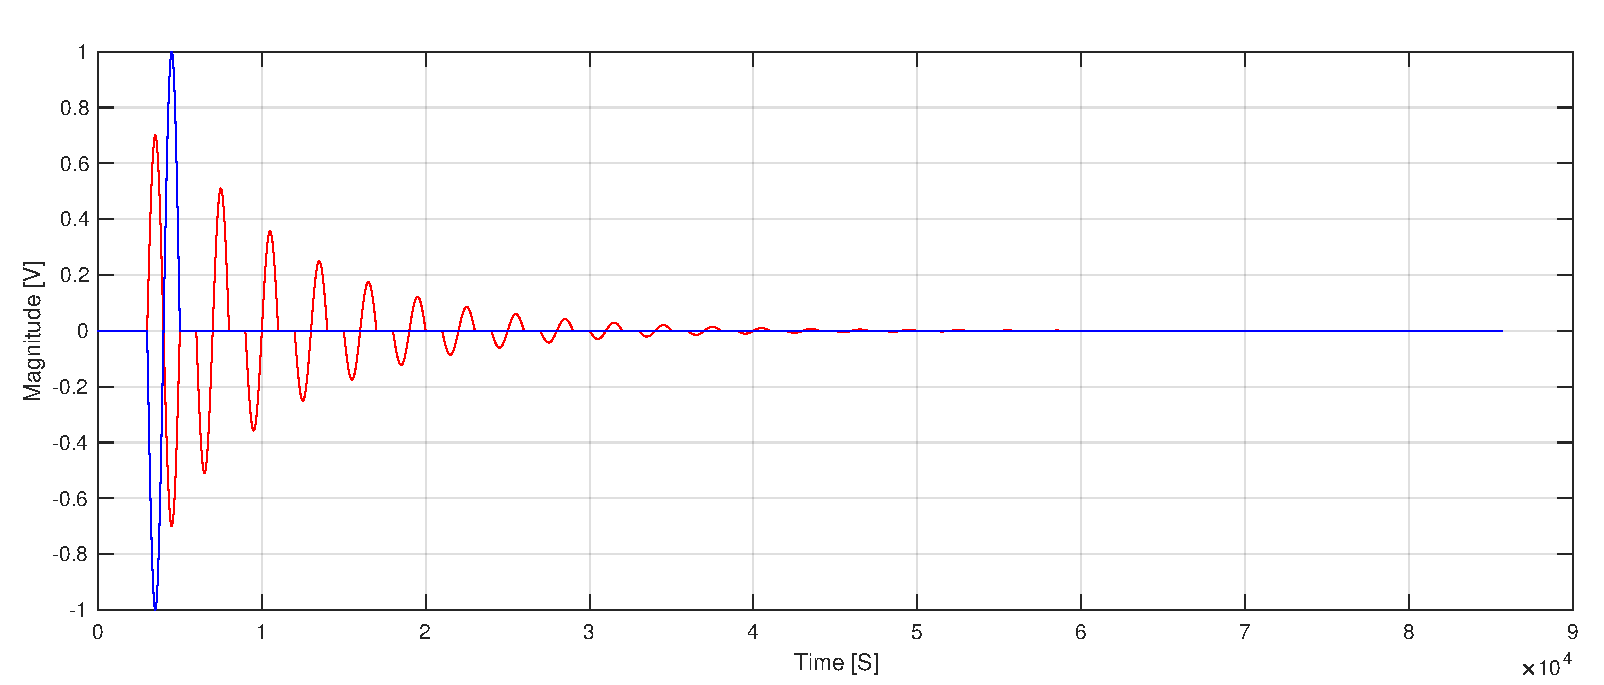
\includegraphics[width=0.7\textwidth]{delay}
	\caption{The plot shows the result for the \autoref{code:delay_sim}}
	\label{fig:delay_plot}
\end{figure}



Applying one sinus round in the \gls{reverb}  effect gives the following result \autoref{fig:delay_plot}. The MATLAB simulation code is included in \autoref{app:reverb} \autoref{code:reverb_sim}.
\begin{figure}[htbp]
	\centering
	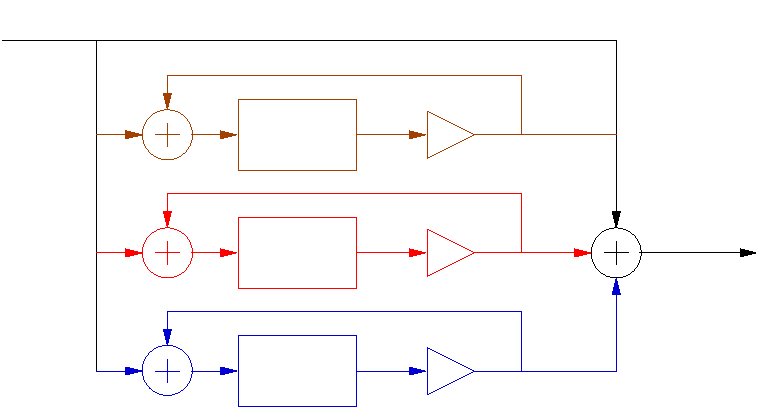
\includegraphics[width=0.6\textwidth]{reverb}
	\caption{The plot shows the result for the \autoref{code:reverb_sim}}
	\label{fig:reverb_plot}
\end{figure}

\newpage
\subsection{implementation}
This section will design the assembly code, where the implementation method is very imported to do the program as efficiency as possible. The delay for example can be done in several ways where ether the data is moved or the pointer is moved, but if it is the data which is moved and there is 1000 data samples, it will require 1000 clock cycles because each data sample needs to be moved alone. If the pointer is moved it will only require one cycles for moving the input pointer and one cycles to move the output pointer, so the delay will be designed as a ring buffer where the input and output pointer is moved. 
The .... only have three circular data buffers size register, where buffer register BK03 will be used to delay samples. \gls{reverb} have the longest delay time, so the data buffers size will be calculated in this section. First the time between 2 samples needs to be calculated, and the calculation is done as following \autoref{eq:sample_time}

\begin{subequations}\label{eq:sample_time}
    \begin{equation}
t_s=\frac{1}{f_s}
    \end{equation}
\centering
$\Updownarrow$
    \begin{equation}
\SI{22.7}{\micro\second}=\frac{1}{\SI{44100}{\hertz}}
    \end{equation}
\end{subequations}

According to \autoref{tab:reverb_delay} the longest delay time is \SI{41}{\milli\second} and as calculated in \autoref{eq:sample_time} the time between samples is \SI{22.7}{\micro\second}. To calculate the number of needed samples in the buffer is done as following \autoref{eq:sample_number}

\begin{subequations}\label{eq:sample_number}
    \begin{equation}
s=\frac{delay}{t_s}+1
    \end{equation}
\centering
$\Updownarrow$
    \begin{equation}
1807=\frac{\SI{41}{\milli\second}}{\SI{22.7}{\micro\second}}+1
    \end{equation}
\end{subequations}

Convertet to hex, the data buffers size register shall have a size of 0x70F and the memory over view will be as following \autoref{fig:reverb_mem_map}

\begin{figure}[htbp]
	\centering
\begin{picture}(0,0)%
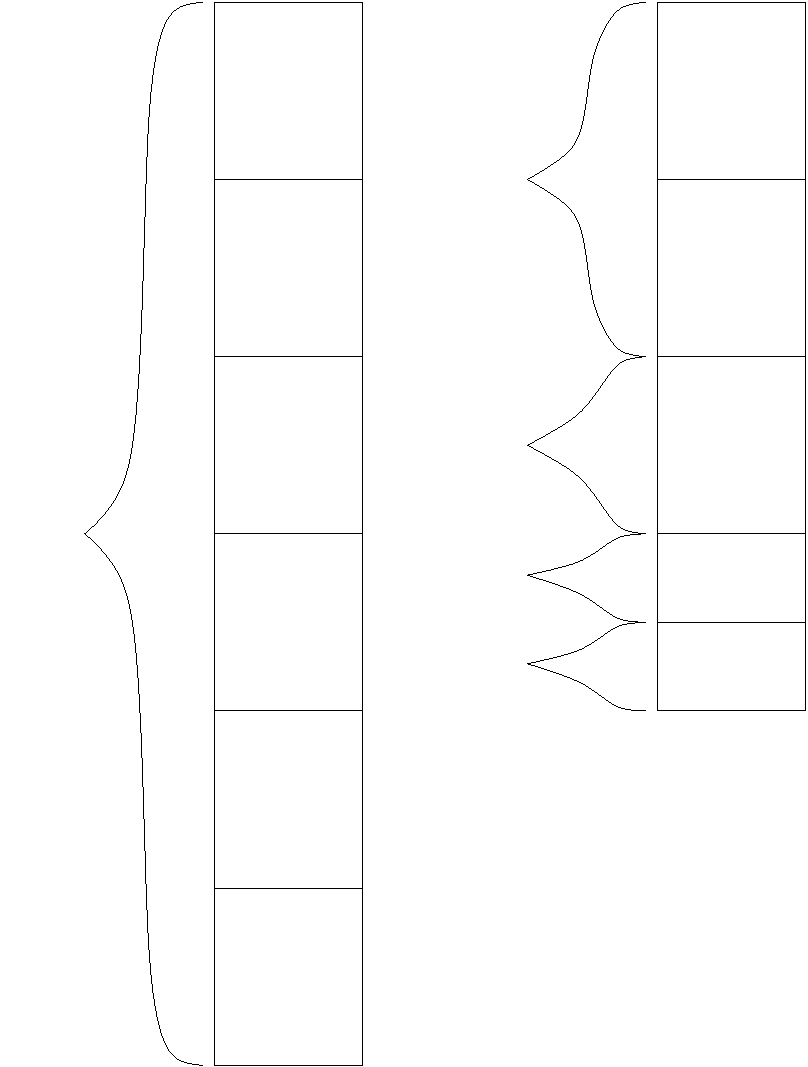
\includegraphics{Reverb_mem.pdf}%
\end{picture}%
\setlength{\unitlength}{4144sp}%
%
\begingroup\makeatletter\ifx\SetFigFont\undefined%
\gdef\SetFigFont#1#2#3#4#5{%
  \reset@font\fontsize{#1}{#2pt}%
  \fontfamily{#3}\fontseries{#4}\fontshape{#5}%
  \selectfont}%
\fi\endgroup%
\begin{picture}(6147,8124)(6241,-7498)
\put(9631,-4471){Coeff}%
\put(8101,389){0x0000}%
\put(8101,-646){0x070E}%
\put(8101,-961){0x070E}%
\put(8101,-1996){0x0E1D}%
\put(8101,-2311){0x0E1E}%
\put(8101,-3346){0x152C}%
\put(8101,-3661){0x152D}%
\put(8101,-4696){0x1C3B}%
\put(8101,-5011){0x1C3C}%
\put(8101,-6046){0x234A}%
\put(8101,-6361){0x234B}%
\put(8101,-7396){0x2A59}%
\put(11476,389){0x2A5A}%
\put(11476,-646){0x3168}%
\put(11476,-961){0x3169}%
\put(11476,-1996){0x3877}%
\put(11476,-2311){0x3878}%
\put(11476,-3346){0x3F86}%
\put(11476,-3661){0x3F87}%
\put(11476,-4336){0x3F96}%
\put(11476,-4696){0x3FA5}%
\put(11476,-4021){0x3F95}%
\put(9496,-3796){All Pass}%
\put(9811,-2806){Tab(X_1[N])}%
\put(9496,-781){All Pass}%
\put(6256,-3526){LPCF}%
\end{picture}%
	\caption{The plot shows the result for the \autoref{code:reverb_sim}}
	\label{fig:reverb_mem_map}
\end{figure}

\newpage
After the Allocation of memory, all the coefficient needs to be calculated to a hex number that can be used in assembly. It is chosen that the point of coefficient all ways are placed as following \autoref{fig:coeff_bit}

\begin{figure}[htbp]
	\centering
\begin{picture}(0,0)%
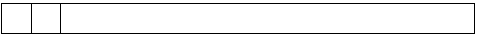
\includegraphics{coeff_bit.pdf}%
\end{picture}%
\setlength{\unitlength}{4144sp}%
%
\begingroup\makeatletter\ifx\SetFigFont\undefined%
\gdef\SetFigFont#1#2#3#4#5{%
  \reset@font\fontsize{#1}{#2pt}%
  \fontfamily{#3}\fontseries{#4}\fontshape{#5}%
  \selectfont}%
\fi\endgroup%
\begin{picture}(3624,274)(6064,352)
\put(6121,434){S}%
\put(7651,434){14 Fraction bit}%
\put(6346,434){X}%
\put(6481,389){\makebox(0,0)[lb]{\smash{{\SetFigFont{14}{16.8}{\rmdefault}{\mddefault}{\updefault}{\color[rgb]{1,0,0},}%
}}}}
\end{picture}%
	\caption{The plot shows the result for the \autoref{code:reverb_sim}}
	\label{fig:coeff_bit}
\end{figure}


Because the point is situated in the front of bit 14 from LSB, the coefficient is allowed to be between 0 and >2 in decimal. The coefficient is therefore multiplied by $2^{14}$ to get the integer and afterwards converted to hex.   The coefficient is done as following \autoref{eq:coeff_cal}

    \begin{equation}\label{eq:coeff_cal}
\text{coeff} \cdot 2^{14}
    \end{equation}

The calculated coefficient to \gls{reverb} is placed in BK47 data buffer register with a memory offset of 0x3F96 and are shown in \autoref{code:reverb_coeff}

\includeCode{main_buffer.asm}{assembly}{31}{46}{The reverb coeff code}{code:reverb_coeff}{code/design/}


\subsection{Reverb Assembly code}
The reverb implementation in Assembly is done by being inspired from the differential equation in \autoref{eq:reverb_eq}. The assembly code is in the file \textit{reverb.asm} and stored in the ZIP file. In the following, each subsection will represent either a subroutine or a macro routine. 

\subsection{The \textit{reverb_pre} Subroutine}

\includeCode{reverb.asm}{assembly}{68}{78}{The reverb coeff code}{code:reverb_coeff}{code/design/}

Since the same buffer is used for all the effects and for different purposes in the same effect, the address of the buffer that contains the needed coefficients for this subroutine is set in the first two lines. The $z^{-ed_n}$ buffer is also moved to the \textit{X_1[N]} buffer. This subroutine is destined to compute the pre \gls{reverb}, the part just before the comb filter. This part is shown in figure \autoref{fig:pre_reverb_block_design}, a fraction of the whole effect diagram in figure \autoref{fig:reverb_block_design}. The idea in the code is to point on different parts of \textit{X_1[N]}  which contains values of \textit{X[N-ed_n]}, the more the pointer has a lower negative number, the bigger the delay. Different values at the pre-calculated delays \textit{ed1}, \textit{ed2}, \textit{ed3} and \textit{ed4} are added together to give $X_{1}[N]$ and then stored in the memory area of  *AR5. \\

\subsection{The \textit{reverb_lpcf} Subroutine}
This subroutine is responsible for computing the equations of the 6 comb filters. The first part is reserved for calculating the different coefficients needed in the calculations, $LD$ and $g$. The beginning of the macro command marks the end of coefficients calculations and the beginning of the equations processing. The choice of a macro implementation here comes after observing big similarities between the six comb filters. The only differences lie in the $b_{i}$ gains, $x_{i}$ values and $d_{i}$ values. This is why they are macro entries. The macro is simply the computation of the equations \ref{eq:reverb_eq_iir1w} to \ref{eq:reverb_eq_iir6w}. The circular buffer AR0 is the one that contains the values of $x_{i}$. AR4 and CDP the pointer which contains the coefficients, gains and delay values.
After the macro section, it is called with the different comb filter settings in a row. 

\subsection{The \textit{reverb_allpass} Subroutine}
The subroutine is the one that takes into account the final part of the \gls{reverb} effect which is the two all-pass filters. It also involves the use of a macro as the previous section since the two all-pass filters have considerable resemblance. Again, *AR0 is used as a buffer pointer for the $x_{i}$ values and *AR4 for the coefficients and the delay values. The other registers and accumulators are used for temporary purposes.
Last but not least, the data is moved to T2 that plays the role of the output. 
Another crucial step is to move the pointer of the AR0 buffer so that in the next iteration the values are not overwritten but inserted in a new slot.
